\mychapter{Sobre o SEB}\label{ch:apendiceC}

Para restringir o acesso a uma atividade VPL no Moodle, foi utilizado o SEB (\textit{Safe Exam Browser}). O arquivo de configuração do SEB está disponível para Windows. Foi utilizado o Windows 10 e a versão do SEB usada neste trabalho foi a 3.7.1.704 (\href{https://safeexambrowser.org/}{safeexambrowser.org}). Essa versão deve ser instalada em todas as máquinas do laboratório. Após gerar o arquivo de configuração do SEB e configurar a atividade VPL conforme descrito, basta clicar duas vezes nesse arquivo e o SEB será executado automaticamente, direcionando para a atividade VPL específica.

\section{Configurando uma atividade no SEB}

Na aba ``\textit{General}'', inclua a URL da atividade VPL do Moodle no campo ``\textit{Start UR}''. Na aba ``Network'', inclua uma URL alternativa para a atividade, como mostrado na Figura \ref{fig:fig_seb_a}. Preste muita atenção à ``\textit{Expression}'' no final da URL \verb|/vpl/*?id=12481*|, onde esse número é a chave da atividade VPL no Moodle. Na aba ``\textit{Exam}'', marque ``\textit{Use Browser Exam Key and Configuration Key}'' e então copie a chave em ``\textit{Browser Exam Key}''. Na aba ``\textit{Config File}'', clique em ``\textit{Save Settings As...}'' para salvar um arquivo no formato SEB~\footnote{Para mais detalhes sobre o SEB, veja \url{https://safeexambrowser.org/windows/win_usermanual_en.html}.}.

A expressão de filtro foi criada pelo Prof. Paulo Henrique Pisani, da UFABC, a quem o autor agradece.

\begin{figure}[!ht]
\centering
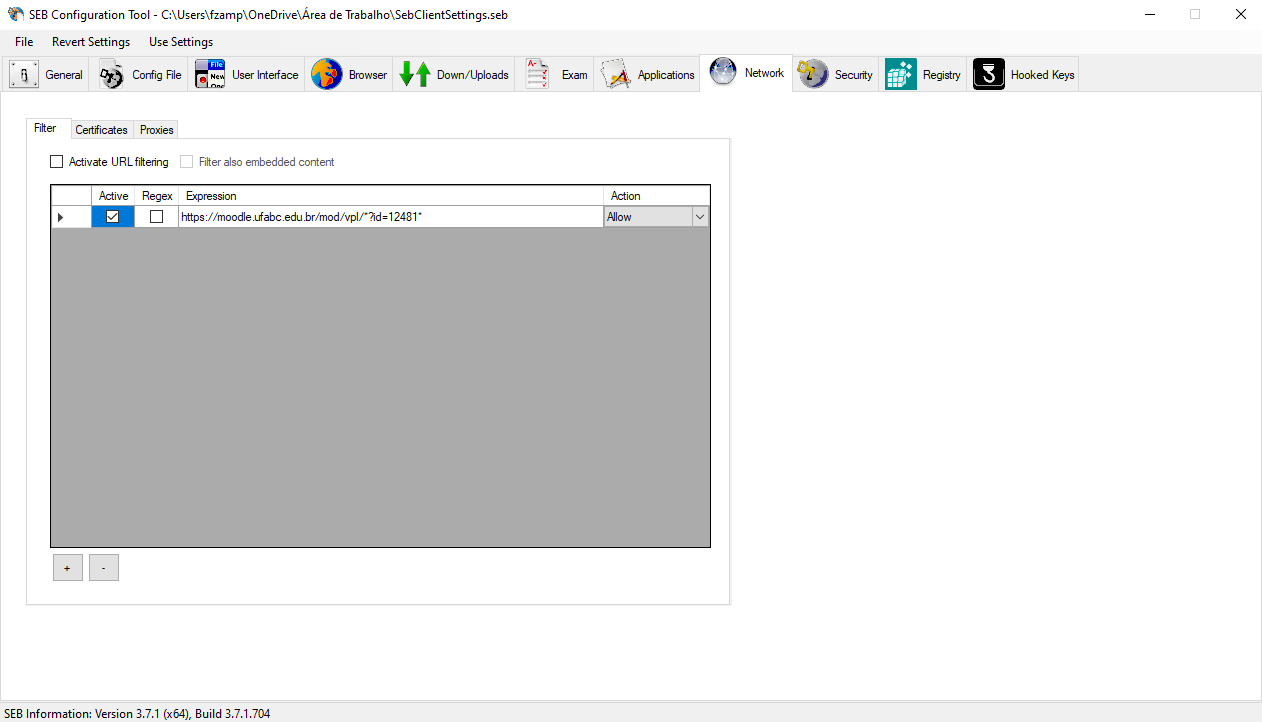
\includegraphics[width=1.0\textwidth]{fig_seb_a.png}
\caption{Captura de tela do SEB mostrando a aba ``Rede'' com restrições de acesso}
\label{fig:fig_seb_a}
\end{figure}

Essa chave deve ser copiada para a atividade VPL do Moodle. No ícone de engrenagem na disciplina do Moodle, vá para ``\textit{Configuration}'', então ``\textit{Submission restrictions}'', ``\textit{Show more}'', defina ``\textit{SEB browser required}'' para SIM e cole a chave em ``\textit{SEB exam Key/s}'', conforme mostrado na Figura \ref{fig:fig_seb_b}.

Se os IPs do laboratório estiverem em uma faixa consecutiva, é possível restringir o acesso à atividade VPL apenas às máquinas do laboratório, incluindo a faixa no campo ``\textit{Allowed submission from net}'' (veja a Figura \ref{fig:fig_seb_b}). Por exemplo, a faixa \verb|111.11.11.1-62| permite todos os IPs entre \verb|111.11.11.1| e \verb|111.11.11.62|. Caso contrário, é necessário incluir cada IP separado por vírgula~\footnote{Para mais detalhes sobre a configuração de IPs na atividade VPL, veja a documentação em \href{https://vpl.dis.ulpgc.es}{vpl.dis.ulpgc.es}.}.

\begin{figure}[!ht]
\centering
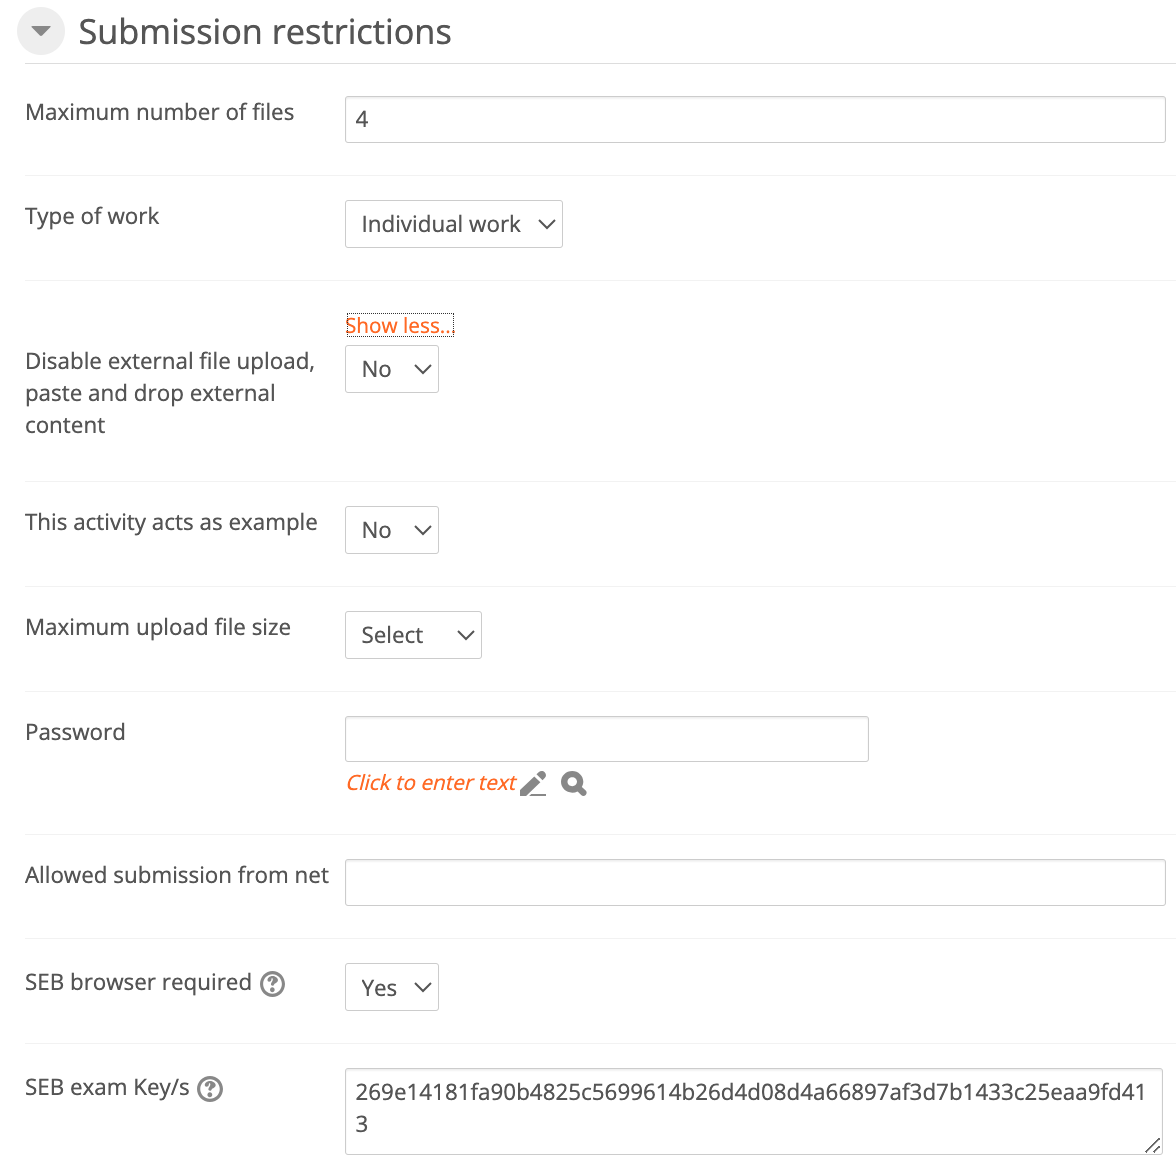
\includegraphics[width=0.8\textwidth]{fig_seb_b.png}
\caption{Captura de tela de uma atividade VPL no Moodle mostrando a chave do SEB}
\label{fig:fig_seb_b}
\end{figure}


\section{Considerações finais}

Este apêndice descreve o uso do SEB para restringir o acesso a uma atividade VPL no Moodle. O arquivo de configuração do SEB foi gerado e aplicado à atividade VPL, garantindo que os estudantes possam acessar a atividade apenas por meio do ambiente seguro do SEB. Isso ajuda a evitar o acesso não autorizado e garante a integridade do processo de avaliação. O uso do SEB, combinado com as restrições de acesso na atividade VPL pelos IP's, fornece uma solução robusta e segura para avaliações de programação online.

